\section{Objet du projet et contexte}
%1-2 pages
%L’objet du projet
%Le contexte général du projet ; son positionnement éventuel dans un projet plus vaste ; synthèse
%des phases antérieures si il y a lieu.
%Son positionnement dans le cycle de vie général du développement des système d’information (
%identification du type de phase à laquelle correspond le projet ; ex : étude préalable,
%spécification d’interface, étude d’architecture technique, réalisation, test, ....)

\subsection{Objet du projet GSTP}
Le projet est une étude préalable de la conception et de l'automatisation
du système d'information du domaine "Gestion du matériel" dans l'entreprise 
GSTP qui est spécialisée dans les activités de terrassement et génie civil.\\

Le but du dossier d'initialisation est de déterminer le périmètre du projet
SI et sa faisabilité, c’est-à-dire de définir ce qui sera inclu
dans le projet, ce qui ne le sera pas et si le projet doit bien être
lancé.\\

D’une part, on estime si les bénéfices attendus seront en proportion des
investissements engagés et du coût prévisionnel du projet SI.  D’autre
part, l’étude préalable détermine également si l’entreprise GSTP est
bien en mesure de mener ce projet à son terme. On cherche en particulier
à savoir si elle dispose des compétences, des ressources et des fonds
nécessaires.\\

On peut dire pour résumer rapidement que le projet consister à urbaniser le
SI de la société GSTP.


\subsection{Contexte général du projet : Présentation de l'entreprise GSTP}

La société GSTP est une SA au capital de 500 M\euro. Elle a à gérer un parc
matériel d'une valeur totale de 300 M\euro et un stock de pièces de
rechanges d'une valeur totale de 100 M\euro.

\subsubsection{Secteur d'activité}
Le projet prend place dans le monde du bâtiment et travaux publiques (GSTP
signifie Génie et Services dans Monde du bâtiment et travaux publiques).


\subsubsection{Organigramme}
L'entreprise est bien structurée et le rôle des différentes entités est clairement défini.\\
On présente ici l'organigramme de la Direction du matériel, sur laquelle
portera le projet.\\

\begin{center}
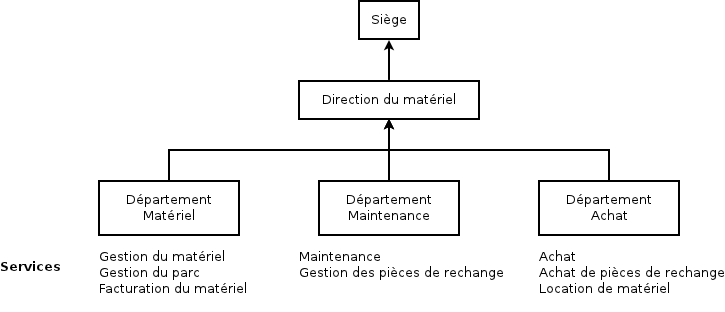
\includegraphics[width=14cm]{\PIXPATH/orga_dir_mat}\hfill\\
\end{center}

La direction matériel est placée sous la direction de la Direction Générale
de la société GSTP. Elle comprend trois département :\\

\begin{description}

\item[Département Matériel] : il gère l'exploitation du matériel de la
société sur les différents chantiers qu'elle mène.
\item[Département Maintenance] : il s'occupe des opérations de maintenance
ordinaires ou exceptionnelles entreprises sur le matériel.
\item[Département Achat] : il a pour charge le renouvellement du parc et
l'achat de nouveaux matériels si nécessaire ; il s'occupe également des
achats de pièces de rechanges.

\end{description}


\subsubsection{Organisation structurelle}

La structure de l'entreprise est basée sur la division siège/chantier :
\begin{description}
\item[Siège]\hfill\\ 
Entité unique où sont regroupés les divers comités de direction de l'entreprise (DG, DRH, DFC, etc.)

\item[Chantier]\hfill\\
Multiples (la société GSTP genre environ 40 chantiers en même temps),
ils sont répartis dans un rayon de 500 km autour du siège.
Les chantiers jouissent d'une certaine autonomie de fonctionnement et
financière par rapport au siège. Les chantiers sont planifiés par la DTEM
au siège de la société. Enfin, le chantier est décrit par une multitude
d'attributs du point de vue gestion (code, nom, localisation, etc.).\\
\end{description}


\subsubsection{Equipement informatique}

Le siège est bien équipé en matériel informatique. En revanche, 
L'équipement des chantiers en matériel informatique est disparate (un tiers
des chantiers est équipé) ; toutefois, l'ensemble sera équipé sur un horizon de
dix mois, ce qui permet d'envisager le projet de manière sereine de ce côté
là.


\subsection{Identification des secteurs de l'entreprise impactés par le projet}

\subsubsection{Activités de l'entreprise}

L'activité principale (travaux publiques) de l'entreprise ne va pas
vraiment être impactée par le projet. En revanche, la manière dont
l'entreprise gère son matériel va se trouver transformée.


\subsubsection{Directions et services}

Au vu de l'objet du projet (automatisation du SI du domaine Gestion du
Matériel), on peut dire que la principale direction de l'entreprise touchée
par le projet sera la Direction du Matériel. Tous les départements de cette
direction seront également touchés par le projet.\\
La manière dont les chantiers gèrent le matériel sera également impactée.


\subsubsection{Processus et procédures stratégiques}

Toutes les procédures liées au matériel employé par la société seront
touchées par le projet. Cela comprend les procédures suivantes :
\begin{itemize}
\item Renouvellement du matériel
\item Affectation
\item Facturation
\item Maintenance
\end{itemize}

